%!TEX root=../Vorlage_DA.tex
%	########################################################
% 				Allgemeiner Teil (Theorie)
%	########################################################


%	--------------------------------------------------------
% 	Allgmeine Hinweise
%	--------------------------------------------------------
\section{Allgemeiner Teil (Theorie)}

\subsection{Erweiterte Backus-Naur-Form (EBNF)}

Die sogenannte Erweiterte Backus-Naur-Form (EBNF)\footnote{\url{https://de.wikipedia.org/wiki/Erweiterte_Backus-Naur-Form}} ist eine Weiterentwicklung der Backus-Naur-Form (BNF)\footnote{\url{https://de.wikipedia.org/wiki/Backus-Naur-Form}}. Das Anwendungsgebiet der BNF und EBNF ist das definieren von  kontextfreie Grammatiken\footnote{\url{https://de.wikipedia.org/wiki/Kontextfreie_Grammatik}}, welche untere anderem f\"ur Programmiersprachen benutzt werden.

Bei kontextfreier Grammatik wird jeweils ein Nichtterminalsymbol auf eine beliebige Folge von Terminal- bzw. Nichtterminalsymbolen abgeleitet ($V \rightarrow w$). Wenn das Nichtterminalsymbol $V$ in einem anderem Nichtterminalsymbol verwendet wird, wird nicht auf den Kontext geachtet, in welcher das Nichtterminalsymbol $V$ eingebettet ist. Die Regel ist daher kontextfrei.

Vorteile der EBNF gegen\"uber der BNF sind unter anderem:

\begin{itemize}
  \item einfacheres erstellen von Rekursionen und optionalen Ausdr\"ucken
  \item bessere Lesbarkeit
  \item einfaches und eindeutiges Definieren von Terminalsymbolen
\end{itemize}

\newpage

\subsubsection{Terminalsymbol}

Ein sogenanntes Terminalsymbol\footnote{\url{https://de.wikipedia.org/wiki/Terminalsymbol}} wird nicht weiter zerlegt. Es stellt z.B. eine Zahl, eine Variable oder ein Schlüsselwort (``if'', ``while'', ...) dar.

\begin{lstlisting}[language=EBNF, escapechar=!]
Expr = Term { ( "!\colorbox{highlight}{+}!" | "!\colorbox{highlight}{-}!" ) Term }.
Term = !\colorbox{highlight}{intCon}! { ( "!\colorbox{highlight}{*}!" | "!\colorbox{highlight}{/}!" ) !\colorbox{highlight}{intCon}! }.
\end{lstlisting}

Terminalsymbole werden normalerweise entweder klein geschrieben (z.B. intCon), oder direkt in der Grammatik definiert (z.B. ''+'').

\subsubsection{Nichtterminalsymbol}

Ein Nichtterminalsymbol\footnote{\url{https://de.wikipedia.org/wiki/Nichtterminalsymbol}} besteht aus einem oder mehreren Terminalsymbolen bzw. Nichtterminalsymbolen.

\begin{lstlisting}[language=EBNF, escapechar=!]
!\colorbox{highlight}{Expr}! = !\colorbox{highlight}{Term}! { ( "+" | "-" ) !\colorbox{highlight}{Term}! }.
!\colorbox{highlight}{Term}! = intCon { ( "*" | "/" ) intCon }.
\end{lstlisting}

Nichtterminalsymbole werden normalerweise gro\ss{} geschrieben. In diesem Beispiel stellen ``Expr'' und ``Term'' Nichtterminalsymbole dar, welche wiederum von anderen Nichtterminalsymbolen verwendet werden k\"onnen.

\subsubsection{Produktionsregel}

Die Produktionsregel\footnote{\url{https://de.wikipedia.org/wiki/Produktionsregel}} ist eine Regel, welche angibt wie aus W\"ortern neue W\"orter produziert werden.

\begin{lstlisting}[language=EBNF, backgroundcolor=\color{highlight}]
Expr = Term { ( "+" | "-" ) Term }.
Term = intCon { ( "*" | "/" ) intCon }.
\end{lstlisting}

Die Produktionsregel gibt an wie z.B. das Nichtterminalsymbol ``Expr'' aufgebaut ist. Eine Produktionsregel besteht jeweils aus einem Nichtterminalsymbol auf der linken Seite, und der jeweiligen Regel auf der rechten Seite welches aus Terminal- und Nichtterminalsymbolen aufgebaut ist.

\newpage

\subsubsection{Eindeutigkeit}

Die Grammatik muss so aufgebaut sein, dass es für einen Tokenstrom nur eine eindeutige Möglichkeit gibt diesen zu parsen.\footnote{\url{http://www.iai.uni-bonn.de/III//lehre/vorlesungen/Informatik_I/WS05/Folien/VLWS0506-10.pdf}} Beim Parsen wird ein Tokenstrom in eine andere Darstellung \"uberf\"uhrt, welcher die weitere Verarbeitung erm\"oglicht. Dies kann aber nur dann reproduzierbar funktionieren, wenn der Parser einen bestimmten Tokenstrom nur in einem eindeutigen Weg durchlaufen darf.

\htlParagraph{Mehrdeutige EBNF Regel}

\begin{figure}[h]
\centering
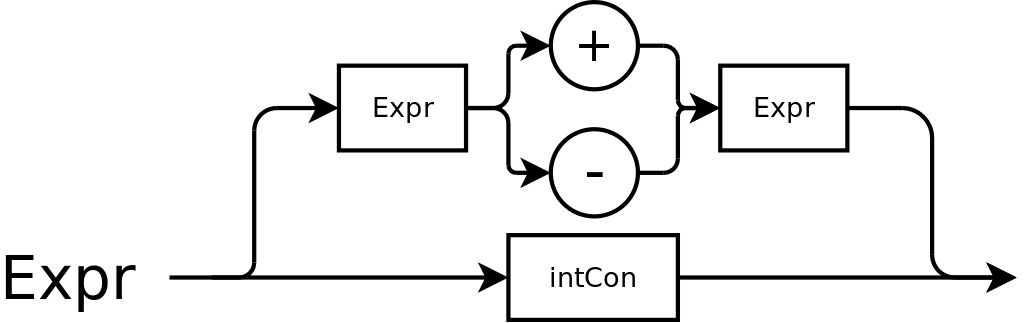
\includegraphics[width=0.6\textwidth]{./media/images/compiler/ambiguity_wrong.png}
\caption{Mehrdeutige EBNF Regel f\"ur einen Ausdruck}
\label{compiler_ambiguity_wrong}
\end{figure}

\begin{lstlisting}[language=EBNF]
Expr = intCon | Expr ( "+" | "-" ) Expr.
\end{lstlisting}

Der Ausdruck $1-2+5$ kann mit dieser EBNF Regel auf mehreren Arten gelöst werden. Es liegt also eine Mehrdeutigkeit vor. Der Ausdruck $1-2+5$ kann dabei sowohl als $(1-2)+5$, aber auch als $1-(2+5)$ geparst werden.

\begin{figure}[h]
\centering
\begin{tabular}{ c | c }
  $(1-2)+5=4$ & 
  $1-(2+5)=-6$ \\
  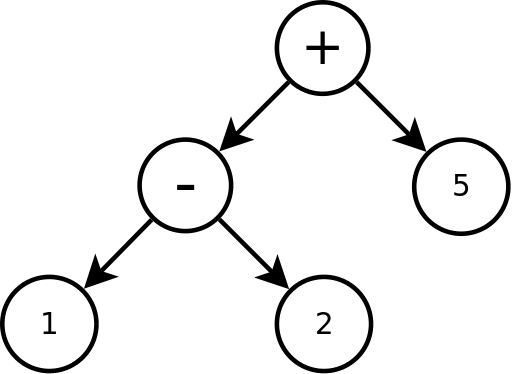
\includegraphics[width=0.2\textwidth]{./media/images/compiler/ambiguity_tree_correct.png} & 
  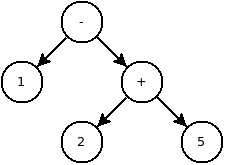
\includegraphics[width=0.2\textwidth]{./media/images/compiler/ambiguity_tree_wrong.png} \\
\end{tabular}
\caption{Es gibt mehrere M\"oglichkeiten diese EBNF-Regel zu durchlaufen}
\label{compiler_ambiguity_wrong_possible_ways}
\end{figure}

\htlParagraph{Eindeutige EBNF Regel}

\begin{figure}[h]
\centering
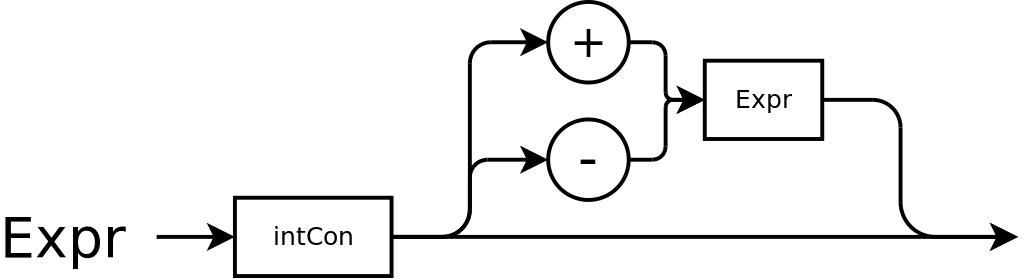
\includegraphics[width=0.6\textwidth]{./media/images/compiler/ambiguity_correct.png}
\caption{Eindeutige EBNF Regel f\"ur einen Ausdruck}
\label{compiler_ambiguity_correct}
\end{figure}

\begin{lstlisting}[language=EBNF]
Expr = intCon [ ( "+" | "-" ) Expr ].
\end{lstlisting}

Der Ausdruck $1-2+5$ kann mit dieser EBNF Regel nur mehr auf eine Art gelöst werden. Dabei werden die Operatoren links-assoziativ behandelt. Der Ausdruck $1-2+5$ wird als $(1-2)+5$ ausgewertet, was mathematisch den korrekten Weg darstellt.

\subsubsection{EBNF-Beispiele}

\begin{figure}[h]
\centering
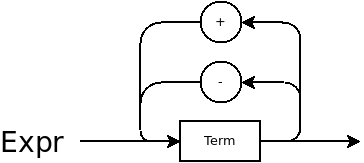
\includegraphics[width=0.5\textwidth]{./media/images/compiler/ebnf_expr.png}
\caption{Grafische Darstellung der EBNF Regel f\"ur einen Ausdruck}
\label{compiler_ebnf_expr}
\end{figure}

\begin{lstlisting}[language=EBNF]
Expr = Term { ( "+" | "-" ) Term }.
\end{lstlisting}

Eine Expression\footnote{\url{https://de.wikipedia.org/wiki/Ausdruck_(Programmierung)}} besteht dabei aus einem Term, und dann optional wiederum aus einem ``+'' oder ``-'' gefolgt von einem weiterem Term.

\begin{figure}[h]
\centering
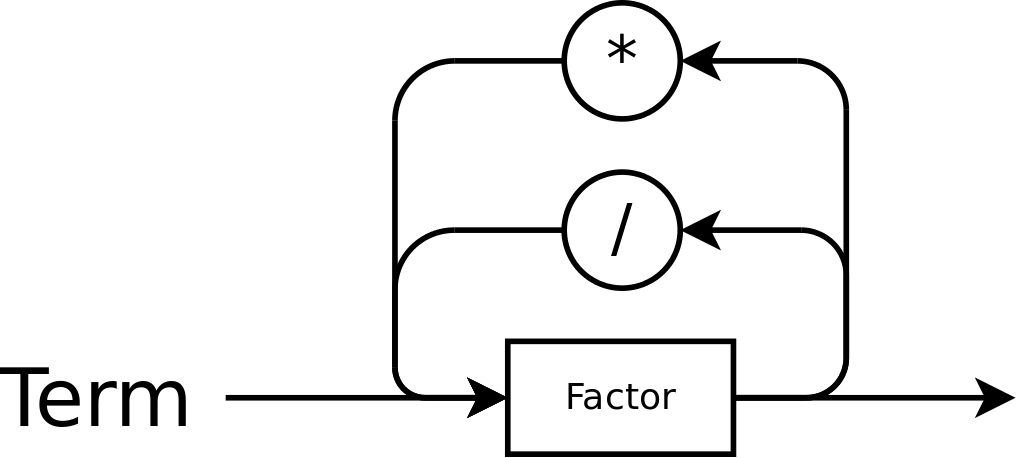
\includegraphics[width=0.5\textwidth]{./media/images/compiler/ebnf_term.png}
\caption{Grafische Darstellung der EBNF Regel f\"ur einen Term}
\label{compiler_ebnf_term}
\end{figure}

\begin{lstlisting}[language=EBNF]
Term = Factor { ( "*" | "/" ) Factor }.
\end{lstlisting}

Das Nichtterminalsymbol Term stellt wiederum eine Produktionsregel dar, welche aus einem Faktor, und dann optional wiederum aus einem ``*'' oder ``/'' gefolgt von einem weiteren Faktor besteht.

Durch solche einfachen Regeln können z.B.: mathematische Regeln wie Punkt vor Strich eindeutig und korrekt in einen Syntaxbaum übersetzt werden.

Diese Produktionsregeln k\"onnen dabei beliebige Komplexit\"at aufweisen, und reichen von einfachen Ausdr\"ucken \"uber den Aufbau des Variablenbezeichners bis zu umfangreichen Zuweisungsoperatoren in allen m\"oglichen Varianten.

\begin{figure}[h]
\centering
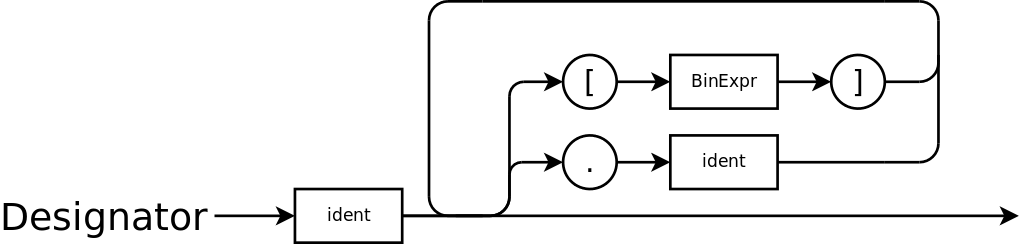
\includegraphics[width=\textwidth]{./media/images/compiler/ebnf_designator.png}
\caption{Grafische Darstellung der EBNF Regel f\"ur einen Variablenbezeichner}
\label{compiler_ebnf_designator}
\end{figure}

\begin{lstlisting}[language=EBNF]
Designator = ident { "." ident | "[" BinExpr "]" }.
\end{lstlisting}

%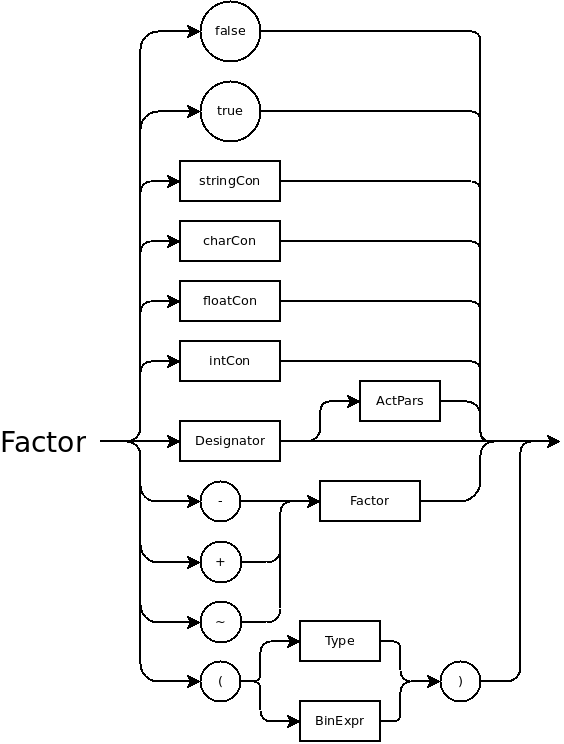
\includegraphics[width=0.6\textwidth]{./media/images/compiler/ebnf_factor.png}

\newpage
\subsection{Lexikalische Analyse - Scanner}

Bei der lexikalischen Analyse zerlegt der sogenannt Scanner\footnote{\url{https://de.wikipedia.org/wiki/Tokenizer}} den Zeichenstrom in einen sogenannten Tokenstrom. Ein Token\footnote{\url{https://de.wikipedia.org/wiki/Token_(\%C3\%9Cbersetzerbau)}} stellt dabei eine logische Einheit dar (z.B.: eine Variable, oder ein Operatorzeichen), und wird nicht mehr weiter zerlegt (Terminalsymbol).

\htlParagraph{Zeichenstrom}

Der Scanner bekommt einen Zeichenstrom, welcher aus einzelnen Zeichen besteht. Ein Zeichen ist z.B. ein Buchstabe, eine Zahl oder Sonderzeichen wie ``='', oder ``+''.

\begin{figure}[h]
\centering
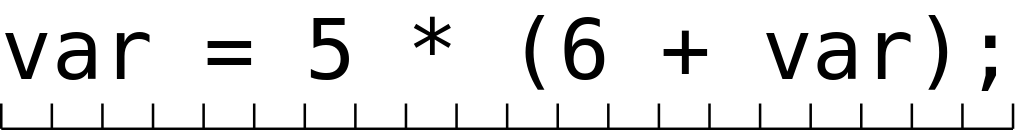
\includegraphics[width=0.6\textwidth]{./media/images/compiler/input_characterstream.png}
\caption{M\"oglicher Eingabedatenstrom aus einzelnen Zeichen}
\label{compiler_input_characterstream}
\end{figure}

\htlParagraph{Resultierender Tokenstrom}

Aus diesem Zeichenstrom werden dann die Tokens extrahiert, welche dann die sogenannten Terminalsymbole in der EBNF bzw. BNF darstellen. Tokens k\"onnen dabei aus 1. oder mehreren Zeichen bestehen.

Manche Tokens wie z.B. Variablen oder Konstanten besitzen au\ss{}er der Tokennummer(welche definiert, um welchen Token es sich handelt) des-weiteren noch einen Tokenwert, mit dem sp\"ater z.B. der Variablenname, oder der Wert einer Variable ausgelesen werden kann.

\begin{figure}[h]
\centering
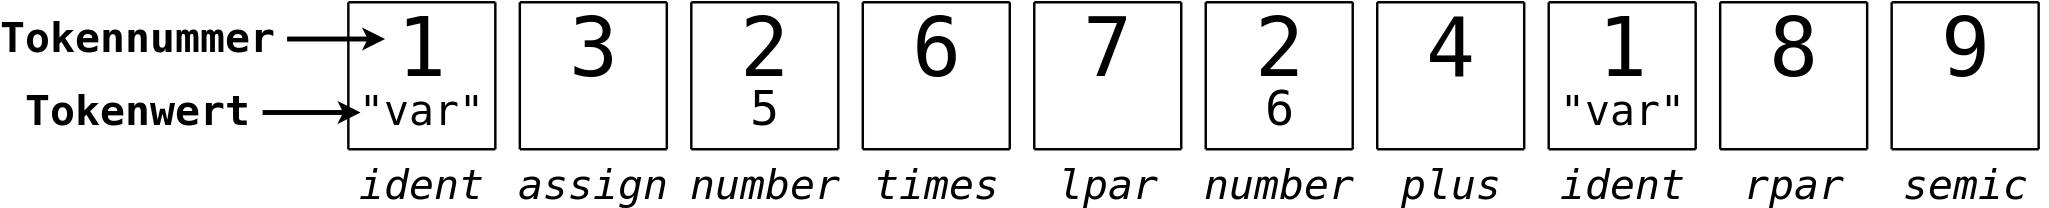
\includegraphics[width=\textwidth]{./media/images/compiler/scanner_tokenstream.png}
\caption{Tokenstrom, welcher aus den Eingabedaten generiert wird}
\label{compiler_scanner_tokenstream}
\end{figure}

\subsection{Syntaxanalyse - Parser}

Der Parser\footnote{\url{https://de.wikipedia.org/wiki/Parser}} wandelt danach den Tokenstrom in einen Syntaxbaum um, welcher das Programm repräsentiert.

Es gibt verschiedene Verfahren um dies zu bewerkstelligen. Wir verwenden f\"ur unser Projekt Coco/R\footnote{\url{https://de.wikipedia.org/wiki/Coco/R}}, welcher einen LL(k)\footnote{\url{https://de.wikipedia.org/wiki/LL(k)-Grammatik}} Parser implementiert, wobei im Normalfall $k = 1$ ist. Falls $k > 1$ ist, muss f\"ur diesen Fall eine eigene Funktion implementiert werden, welche entscheidet wie der Parser weiterarbeiten soll.

Ein LL(1) Parser arbeitet dabei so, dass er jeweils um 1. Token nach vorne schaut, und mithilfe dieser Information den weiteren Parservorgang steuert.

% http://amor.cms.hu-berlin.de/~kunert/papers/lr-analyse/

\newpage

\htlParagraph{Syntaxbaum}

Der Parser \"ubersetzt den Tokenstrom in einem sogenannten Syntaxbaum\footnote{\url{https://de.wikipedia.org/wiki/Syntaxbaum}}, welcher die Struktur des Programmes repr\"asentiert. Dieser umfasst alle Terminal wie auch Nichtterminalsymbole, und zeigt auf wie die EBNF-Regeln aufeinander aufgebaut sind.

\begin{figure}[h]
\centering
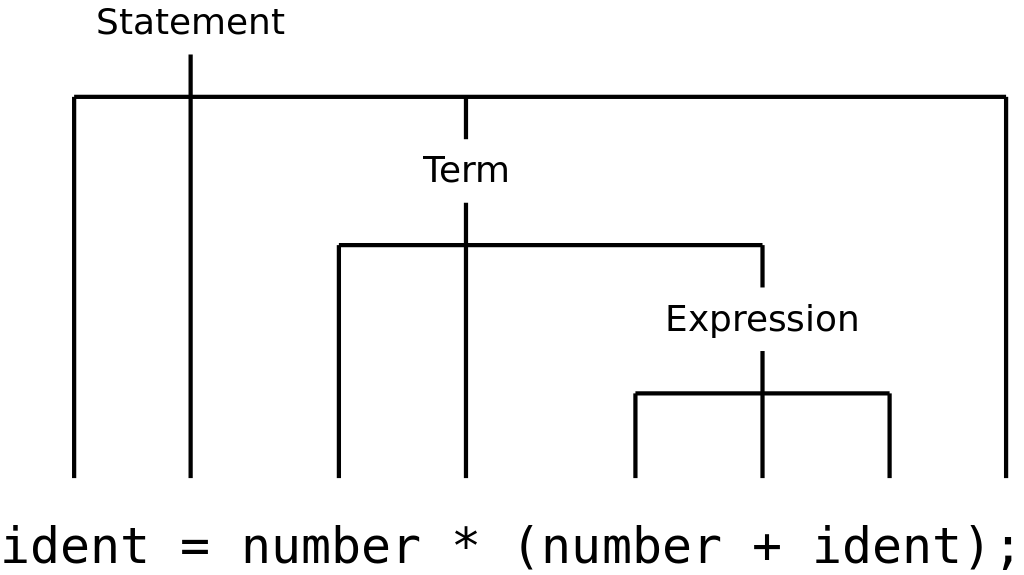
\includegraphics[width=0.5\textwidth]{./media/images/compiler/parser_syntaxtree.png}
\caption{Syntaxbaum welcher aus dem Tokenstrom generiert werden kann}
\label{compiler_parser_syntaxtree}
\end{figure}

\subsection{Abstrakter Syntaxbaum}

Der ``allgemeine'' Syntaxbaum enth\"alt viele unn\"otigen Daten, welche beim abstrakten Syntaxbaum\footnote{\url{https://de.wikipedia.org/wiki/Abstrakter_Syntaxbaum}} nicht mehr vorhanden sind. Der Abstrakte Syntaxbaum stellt somit eine Baumrepr\"asentation der wesentlichen Syntax eines Programmes dar.

Der abstrakte Syntaxbaum wird explitzit w\"ahrend des Parsens gebaut; z.B. mithilfe einer attributierte Gramatik, welche den abstrakten Syntaxbaum an bestimten Stellen innerhalb der EBNF erweitert.

\begin{figure}[h]
\centering
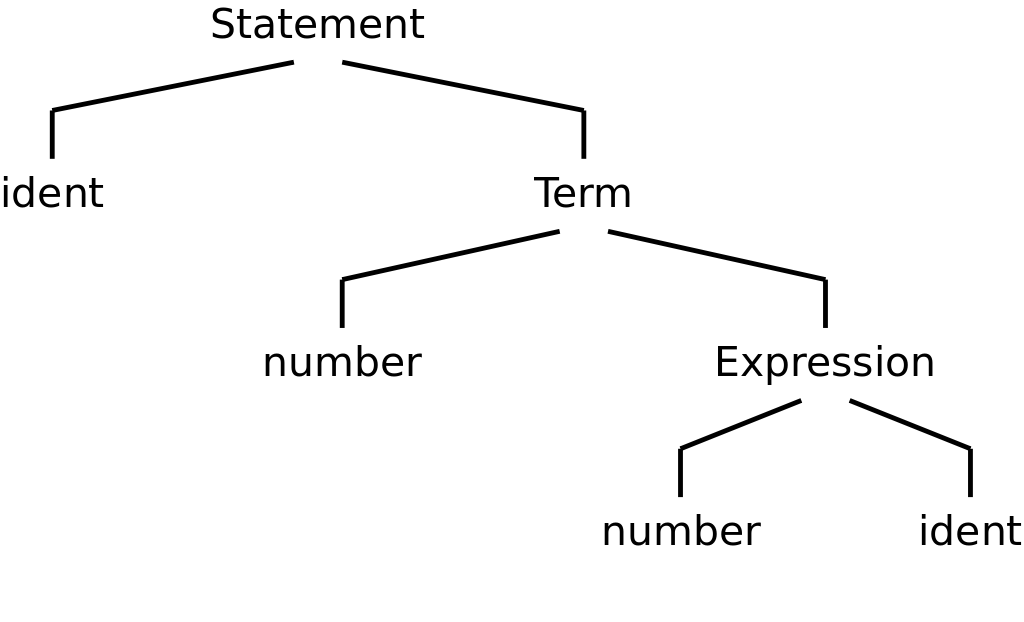
\includegraphics[width=0.5\textwidth]{./media/images/compiler/abstract_syntaxtree.png}
\caption{Abstrakter Syntaxbaum welcher nur mehr notwendige Daten enth\"alt}
\label{compiler_parser_syntaxtree}
\end{figure}

\subsubsection{homogene und heterogene Syntaxbäume}

Der Abstrakte Syntaxbaum kann entweder aus einheitlichen Knoten (homogen) oder aus verschiedenen Knoten (heterogen) aufgebaut sein.\footnote{\url{https://wiki.fernuni-hagen.de/eclipse/index.php/Abstract_Syntax_Tree_(AST)\#Konzept_des_Syntaxbaums}}

\subsection{Attributierte Gramatik}

%\footnote{\url{https://de.wikipedia.org/wiki/Attributgrammatik}}
Bei der attributierten Gramatik\footnote{\url{http://steffenpingel.de/files/papers/ast.pdf}} werden Berechnungsvorschriften direkt in die Gramatik eingef\"ugt. Dadurch k\"onnen w\"ahrend des Parsens unter anderem Syntaxbedingungen wie z.B. Typpr\"ufungen durchgef\"uhrt werden.

In Coco/R werden diese Berechnungsvorschriften mit ``(.'' eingeleitet und mit ``.)'' beendet. Zwischen diesen Klammern befindet sich dann der Quellcode, welcher ausgef\"uhrt wird, falls der Parser den Ausdruck durchl\"auft.

\htlParagraph{Beispiel}

\begin{lstlisting}[language=EBNF]
Type<out Struct type>
= 
ident     (.  // check if a type with the given name exist
              Obj obj = tab.find(t.val);
              if(obj.kind != Obj.TYPE)
                  SemErr(obj.name + " is not a type");

              type = obj.type; .)
. 
\end{lstlisting}

In diesem Beispiel pr\"uft die Berechnungsvorschrift ob bereits ein Identifier mit dem gew\"ahlten Namen definiert wurde (passiert in der Funktion tab.find(t.val);), und ob der gefundene Identifier ein Typ ist. 

Falls eine dieser Syntaxbedingungen fehlschl\"agt, wird ein semantischer Fehler geworfen. So werden w\"ahrend des Parsens nicht nur Syntaxfehler, sondern auch logische Fehler detektiert (z.B. fehlende Variablendeklaration).

Desweiteren kann durch diese Berechnungsvorschriften ein Abstraker Syntaxbaum aufgebaut werden. Eine EBNF-Regel stellt nicht unbedingt einen Knoten im Abstrakten Syntaxbaum dar, da z.b. Variablendeklarationen oft in sogenannte Symboltabellen gespeichert werden.

\subsection{Symboltabelle}

Die Symboltabelle\footnote{\url{https://de.wikipedia.org/wiki/Symboltabelle}} ist eine Datenstruktur in der Variablen und Funktionsdeklarationen gespeichert werden. Sie umfasst dabei Informationen wie z.b. die Zeilennummer, in der die Variable/Funktion deklariert wurde, die Gr\"o\ss{}e des Datentypes, oder auch den Wert mit welchem die Variable deklariert wurde (Konstanten).

Mithilfe der Symboltabelle wird unter anderem festgestellt, ob eine Variablen deklariert wurde, oder wie viel Speicher f\"ur eine Funktion reserviert werden muss.

%, und l\"ost m\"ogliche Namensprobleme auf.\footnote{\url{https://de.wikipedia.org/wiki/Namensraum}}

%\subsection{Scope}